\documentclass[a4paper]{article}
\usepackage[spanish]{babel}
\usepackage[utf8]{inputenc}
\usepackage[T1]{fontenc}
%\usepackage{charter}   % tipografia
\usepackage{graphicx}
\usepackage{enumerate}
\usepackage{algorithm}
\usepackage{algorithmic}[1]
\usepackage{listings}
\usepackage{booktabs}
\usepackage{color}
\usepackage{indentfirst}
\usepackage{fancyhdr}
\usepackage{latexsym}
\usepackage{lastpage}
\usepackage{subfig}
\usepackage{longtable}
\usepackage[colorlinks=true, linkcolor=black]{hyperref}
%\usepackage{makeidx}
%\usepackage{float}
\usepackage{calc}
\usepackage{amsmath, amsthm, amssymb}
\usepackage{amsfonts}
\usepackage{tabularx}
\usepackage{multirow}
%\usepackage{sectsty}
%\usepackage{charter}
%\usepackage{wrapfig}
%\usepackage{listings}
%\lstset{language=C}
\definecolor{gray}{gray}{0.5}
\definecolor{light-gray}{gray}{0.95}
\definecolor{orange}{rgb}{1,0.5,0}

\usepackage{color} % para snipets de codigo coloreados
\usepackage{fancybox}  % para el sbox de los snipets de codigo

\definecolor{litegrey}{gray}{0.94}

% \newenvironment{sidebar}{%
% 	\begin{Sbox}\begin{minipage}{.85\textwidth}}%
% 	{\end{minipage}\end{Sbox}%
% 		\begin{center}\setlength{\fboxsep}{6pt}%
% 		\shadowbox{\TheSbox}\end{center}}
% \newenvironment{warning}{%
% 	\begin{Sbox}\begin{minipage}{.85\textwidth}\sffamily\lite\small\RaggedRight}%
% 	{\end{minipage}\end{Sbox}%
% 		\begin{center}\setlength{\fboxsep}{6pt}%
% 		\colorbox{litegrey}{\TheSbox}\end{center}}

\newenvironment{codesnippet}{%
	\begin{Sbox}\begin{minipage}{\textwidth}\sffamily\small}%
	{\end{minipage}\end{Sbox}%
		\begin{center}%
		\colorbox{litegrey}{\TheSbox}\end{center}}



\usepackage{fancyhdr}
\pagestyle{fancy}

%\renewcommand{\chaptermark}[1]{\markboth{#1}{}}
\renewcommand{\sectionmark}[1]{\markright{\thesection\ - #1}}

\fancyhf{}

\fancyhead[LO]{Sección \rightmark} % \thesection\ 
\fancyfoot[LO]{\small{Ricardo Colombo, Carolina Lang, Jonás Levy Alfie}}
\fancyfoot[RO]{\thepage}
\renewcommand{\headrulewidth}{0.5pt}
\renewcommand{\footrulewidth}{0.5pt}
\setlength{\hoffset}{-0.8in}
\setlength{\textwidth}{16cm}
%\setlength{\hoffset}{-1.1cm}
%\setlength{\textwidth}{16cm}
\setlength{\headsep}{0.5cm}
\setlength{\textheight}{25cm}
\setlength{\voffset}{-0.7in}
\setlength{\headwidth}{\textwidth}
\setlength{\headheight}{13.1pt}

\renewcommand{\baselinestretch}{1.1}  % line spacing


% \setcounter{secnumdepth}{2}
\usepackage{underscore}
\usepackage{caratula}
\usepackage{url}
\usepackage{float}

\newcommand{\cod}[1]{{\tt #1}}
\newcommand{\negro}[1]{{\bf #1}}
\newcommand{\ital}[1]{{\em #1}}
\newcommand{\may}[1]{{\sc #1}}
\newcommand{\tab}{\hspace*{2em}}

\newcommand{\apply}[1]{\applyParam{#1}{}}
\newcommand{\applyParam}[2]{{$\rightarrow$ #1(#2)}}
\newcommand{\notEmpty}[1]{{#1\apply{count} > 0}}
\newcommand{\laterThan}[1]{{self.Status > #1 $\Rightarrow$}}

\hypersetup{
 pdfstartview= {FitH \hypercalcbp{\paperheight-\topmargin-1in-\headheight}},
 pdfauthor={Grupo},
 pdfsubject={Dise\~{n}o}
}

\lstdefinestyle{customc}{
  backgroundcolor=\color{light-gray},
  belowcaptionskip=1\baselineskip,
  breaklines=true,
  numbers=left,
  xleftmargin=\parindent,
  language=C,
  showstringspaces=false,
  basicstyle=\footnotesize\ttfamily,
  keywordstyle=\bfseries\color{blue},
  commentstyle=\itshape\color{gray},
  identifierstyle=\color{black},
  stringstyle=\color{orange},
}

\lstdefinestyle{customasm}{
  backgroundcolor=\color{light-gray},
  belowcaptionskip=1\baselineskip,
  numbers=left,
  xleftmargin=\parindent,
  language=[x86masm]Assembler,
  keywordstyle=\bfseries\color{blue},
  basicstyle=\footnotesize\ttfamily,
  commentstyle=\itshape\color{gray},
}

\lstset{escapechar=@}


\begin{document}

\newcolumntype{C}{>{\centering\arraybackslash}X}

\thispagestyle{empty}
\materia{Ingeniería de Software I}
\submateria{Primer Cuatrimestre de 2016}
\titulo{Trabajo Práctico II}
%\subtitulo{\emph{Si nos organizamos aprobamos todos...}}
%\grupo{Los heladeros de Gauss}
\integrante{Assenza, Franco}{921/12}{assenza.f@gmail.com}
\integrante{Candioti, Alejandro}{784/13}{amcandio@gmail.com}
\integrante{Colombo, Ricardo}{156/08}{ricardogcolombo@gmail.com}
\integrante{Lang, Carolina}{906/12}{carolinalang93@gmail.com}
\integrante{Levy Alfie, Jon\'as}{081/12}{jonaslevy5@gmail.com}
%\fecha{\date{\currentdate}}

\makeatletter
\renewcommand{\ALG@name}{Algoritmo}

\maketitle
\newpage

\thispagestyle{empty}
\vfill

\thispagestyle{empty}
\vspace{3cm}
\tableofcontents
\newpage

\newenvironment{myindentpar}[1]
{\begin{list}{1}
         {\setlength{\leftmargin}{#1}}
         \item[]
}
{\end{list} }

%\normalsize
\newpage

\section{Modelo conceptual}
\subsection{Condiciones OCL}
\begin{itemize}
		\item	\textbf{Momentos en los cuales se puede redefinir el PM o proveedor de un proyecto:}
	
			Context: Proyecto
			
			\begin{tabular}{ll}
				self.redefiniendoProveedor $\Rightarrow$	& BuscandoProveedor < self.Status $\leq$ ObraEnCurso	\\
				self.redefiniendoPM $\Rightarrow$			& EligiendoPM < self.Status $\leq$ ObraEnCurso			\\
			\end{tabular}

	\item \textbf{Estado del proyecto:}

			Context: Proyecto
			
			\begin{tabular}{ll}
				\laterThan{EligiendoPM}				& \notEmpty{self.supervisaHistorico} and						\\
													& ((self.redefiniendoPM) xor (\notEmpty{self.supervisaActual}))	\\
				
				and \laterThan{DefiniendoAlcance}	& \notEmpty{self.alcance} \\
				
				and \laterThan{BuscandoProveedor}	& \notEmpty{self.proveedorHistorico} and	\\
													& (self.redefiniendoProveedor xor			\\
													& (\notEmpty{self.proveedorActual}))		\\
				
				and \laterThan{FirmandoContratos}	& \notEmpty{contratoCliente(self, self.Solicitante)} and	\\
													& (self.redefiniendoProveedor xor							\\
													& \notEmpty{contratoProveedor(self, self.ProveedorActual)})	\\
				
				and \laterThan{ConsiguiendoFeedback}	& \notEmpty{self.FeedbackProveedor} and	\\
														& \notEmpty{self.FeedbackPM}			\\
			\end{tabular}
			
	\item \textbf{Seguro de caución al día:}
	
			Context: Proyecto
			
			\notEmpty{self.ProveedorActual} and self.Status $\leq$ ObraEnCurso $\Rightarrow$
			
			\begin{tabular}{ll}
				\hfill
				& \notEmpty{self.ProveedorActual.Seguro} and	\\
				& self.ProveedorActual.Seguro.Vencimiento $\geq$ ContratoProveedor(self, self.ProveedorActual).FechaFin	\\
			\end{tabular}
				
	\item \textbf{Los autores de reportes son PM del proyecto:}
		
			Context: Reporte de estado 
			
			\notEmpty{self.Autor.SupervisaHistorico $\rightarrow$ filter(p | p == self.Proyecto)}
	
	\item \textbf{Los puntajes de los agentes se corresponden con los puntajes seg\'un proyectos:}
			
			Context: PM
			
			self.puntaje == self.Asignaciones\applyParam{filter}{Proyecto}
				
				\applyParam{select}{p\|p.FeedbackPM\apply{size} > 0}\applyParam{filter}{FeedbackPM}
				
				\applyParam{filter}{Calificacion}\apply{average}
				
			Context: Proveedor
			
			FALTA HACER ESTE
	
	\item \textbf{Los estados del proyecto pero para el otro lado?}
	\item \textbf{Fechas de los reportes?}
	\item \textbf{Solapamiento de PMs historico?}
	\item \textbf{Solapamiento de proveedores historico?}
	\item \textbf{Porcentaje de las comisiones}
	\item \textbf{Fechas de fin luego de fechas de inicio}
	
\end{itemize}

\newpage

\subsection{Casos de Uso}

En esta sección intentaremos terminar de definir de manera mas precisa y detallada las diferentes interacciones que puedan existir entre nuestro sistema y los diferentes actores. Para ello utilizaremos el modelado con un diagrama de casos de uso.

\begin{figure}[H]
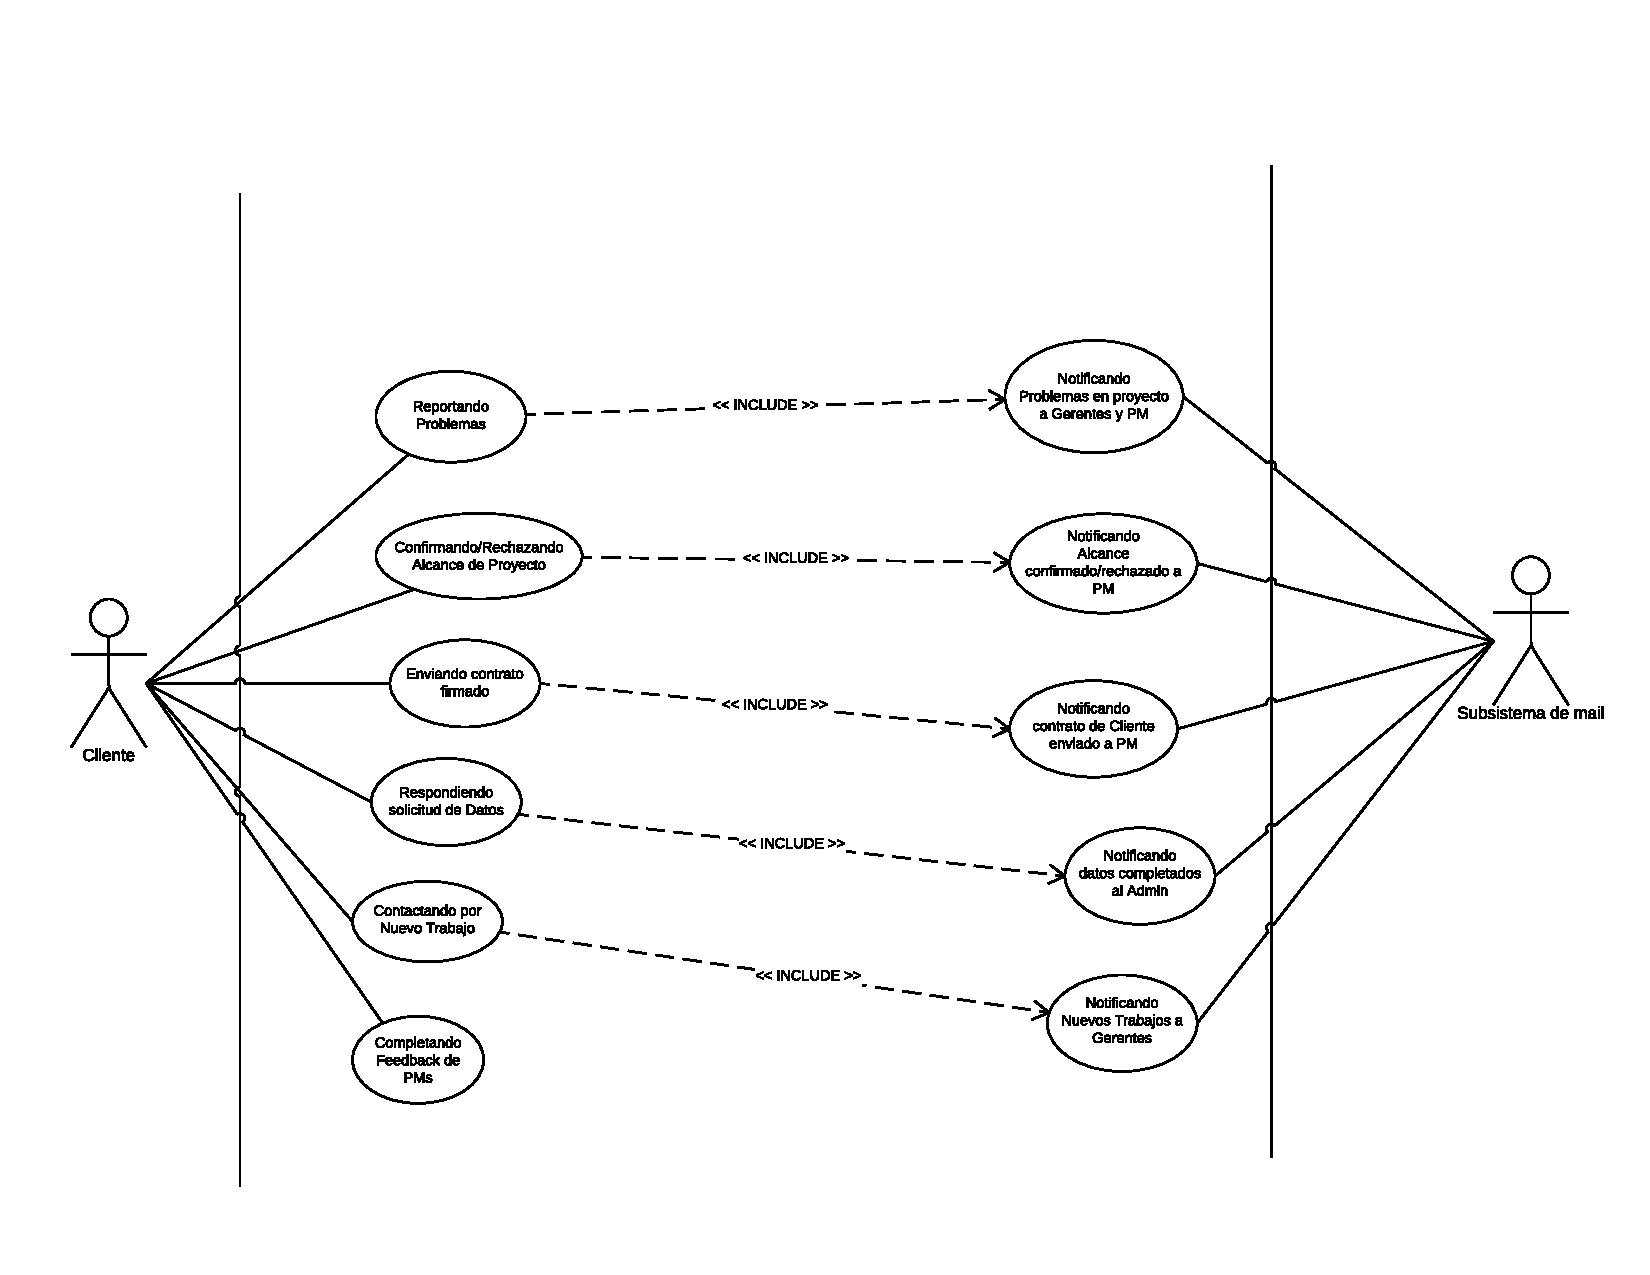
\includegraphics[width=\linewidth]{diag/viejos/cu1.pdf}
\end{figure}
\begin{figure}[H]
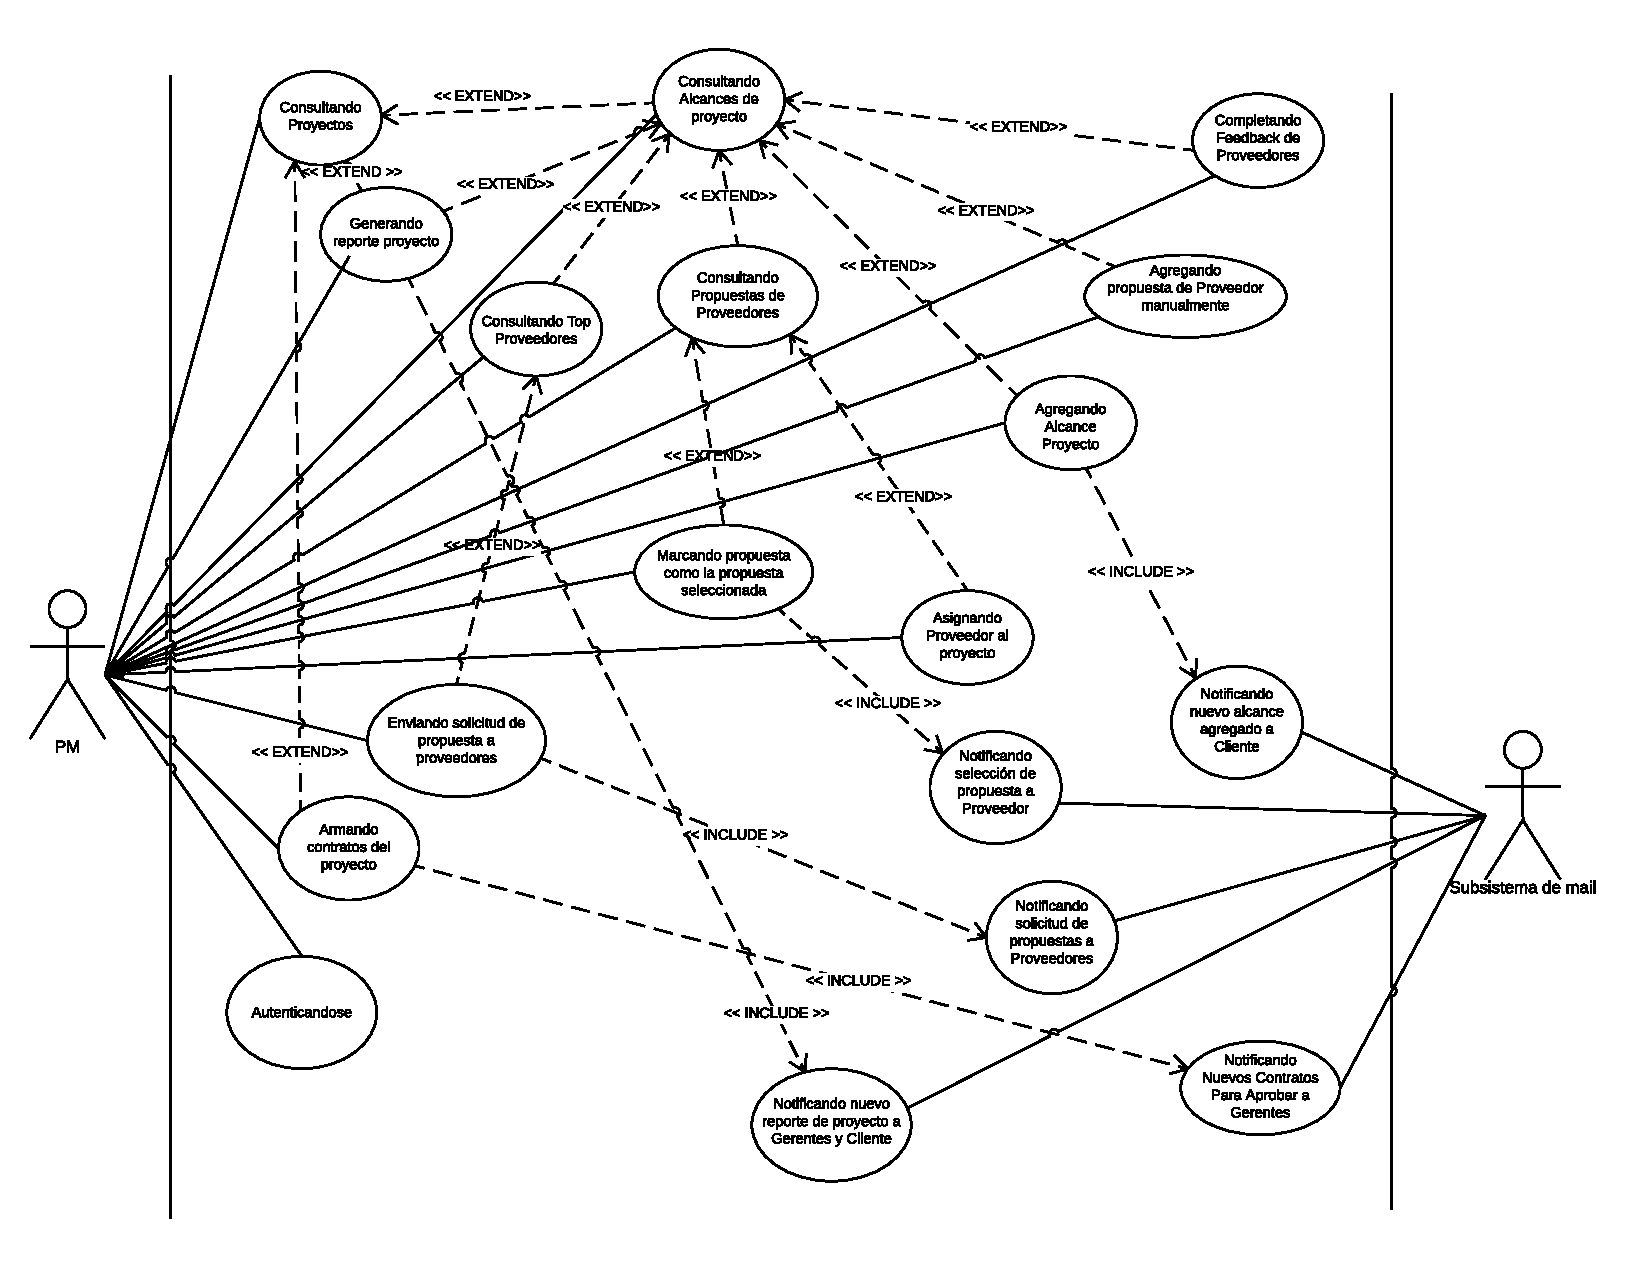
\includegraphics[width=\linewidth]{diag/viejos/cu2.pdf}
\end{figure}
\begin{figure}[H]
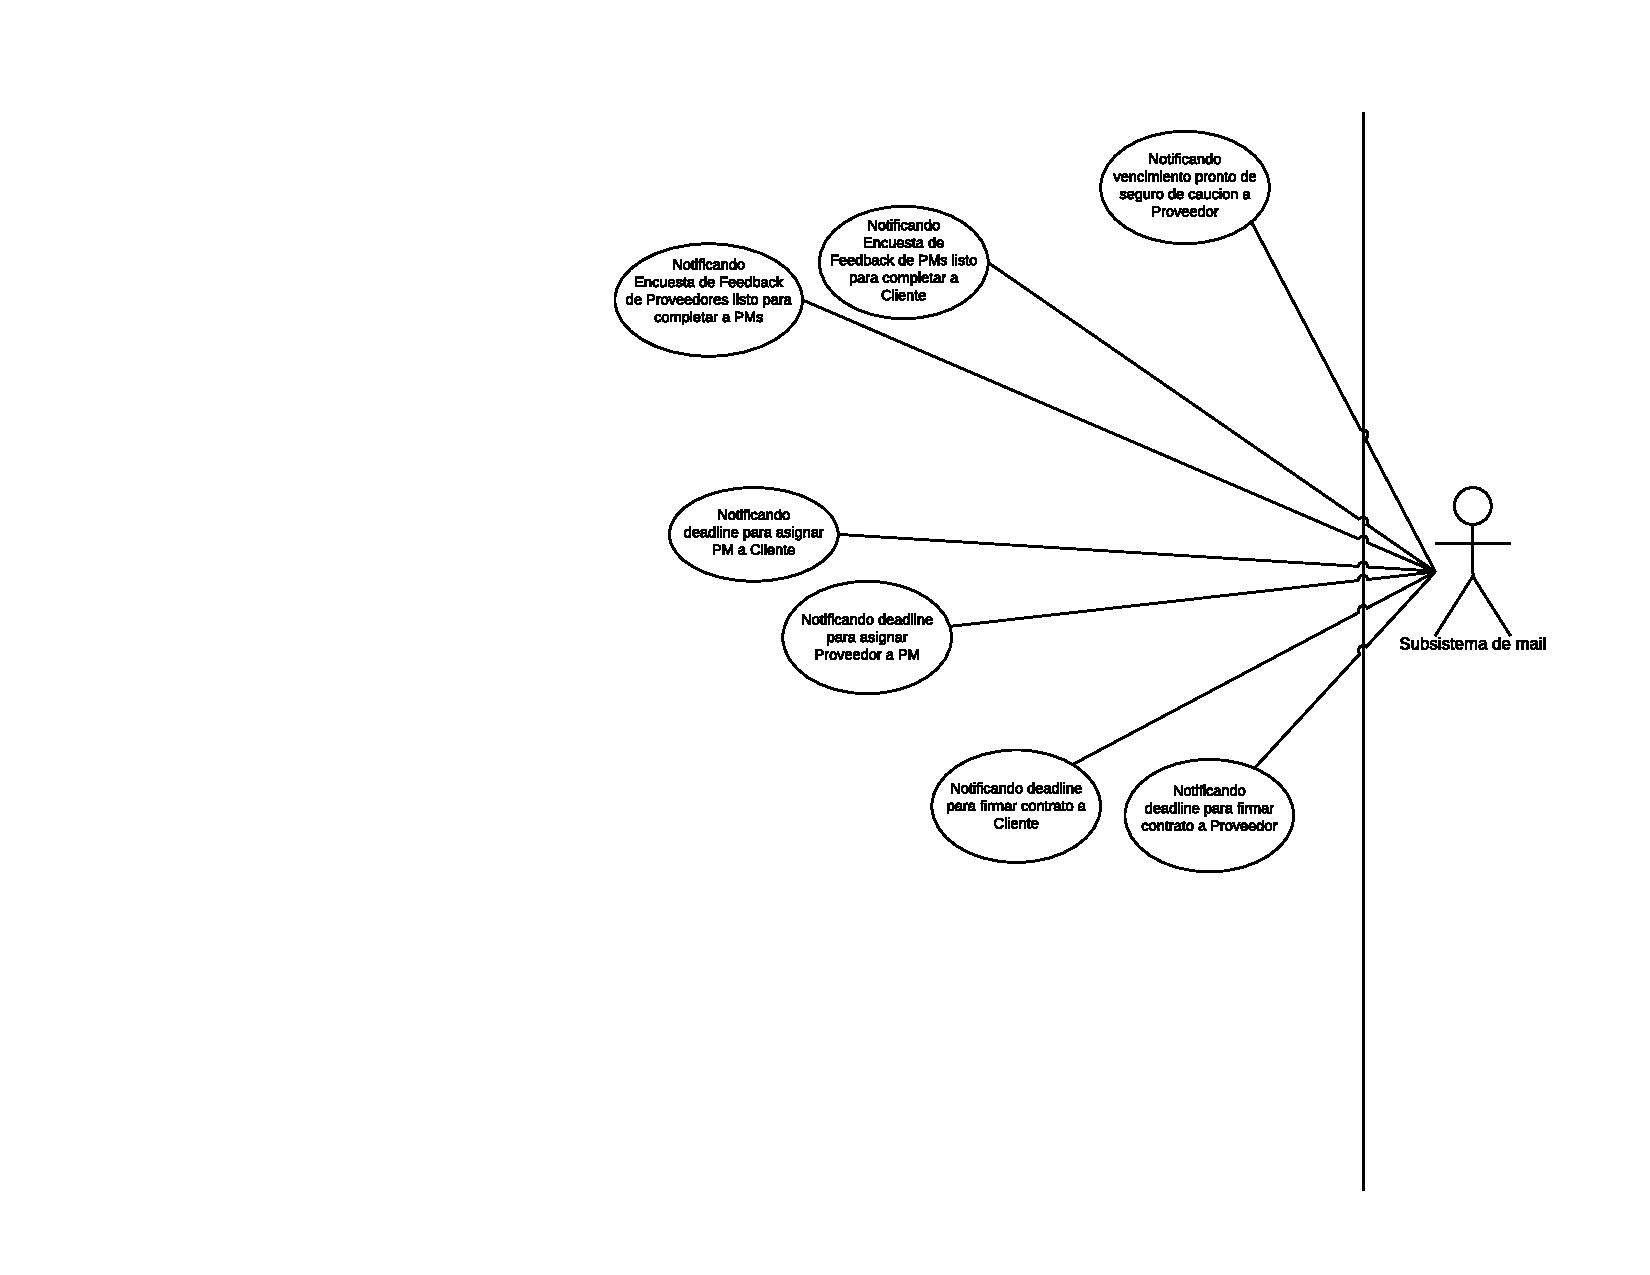
\includegraphics[width=\linewidth]{diag/viejos/cu3.pdf}
\end{figure}
\begin{figure}[H]
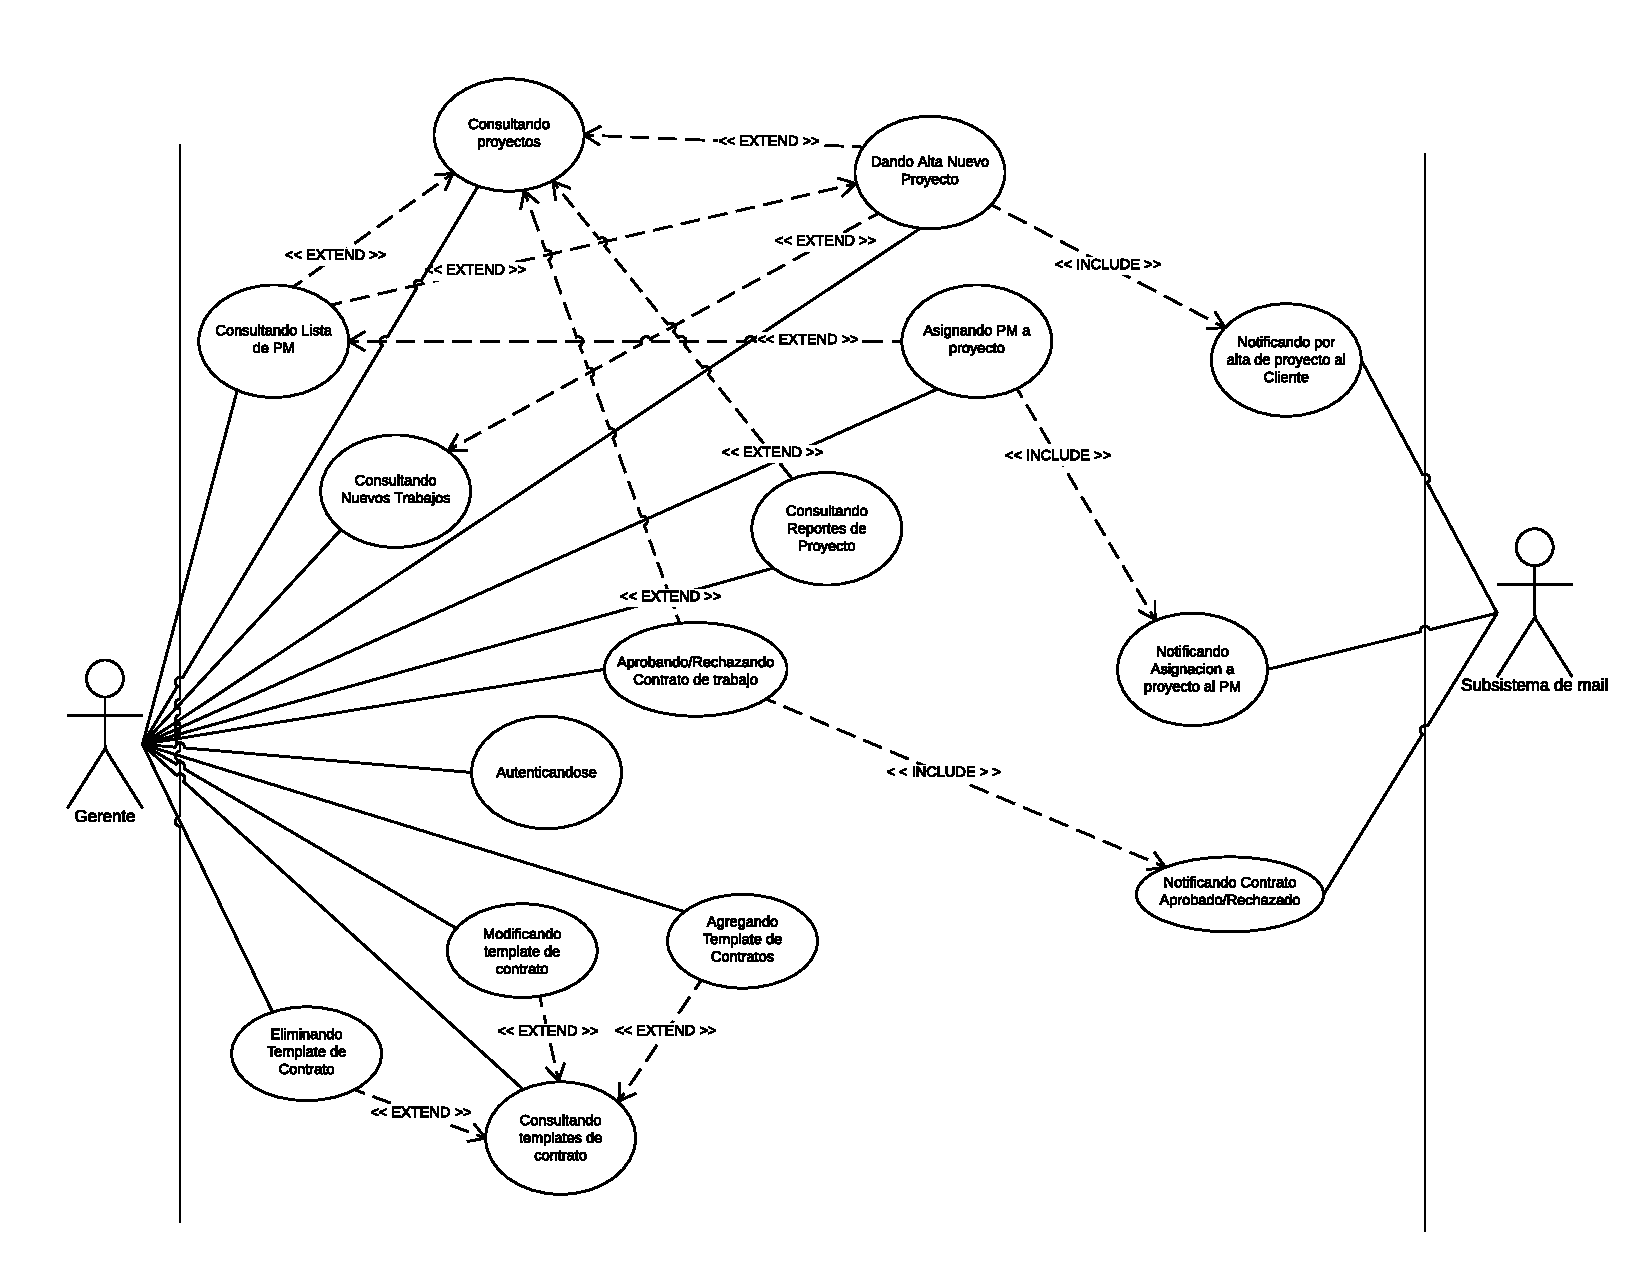
\includegraphics[width=\linewidth]{diag/viejos/cu4.pdf}
\end{figure}
\begin{figure}[H]
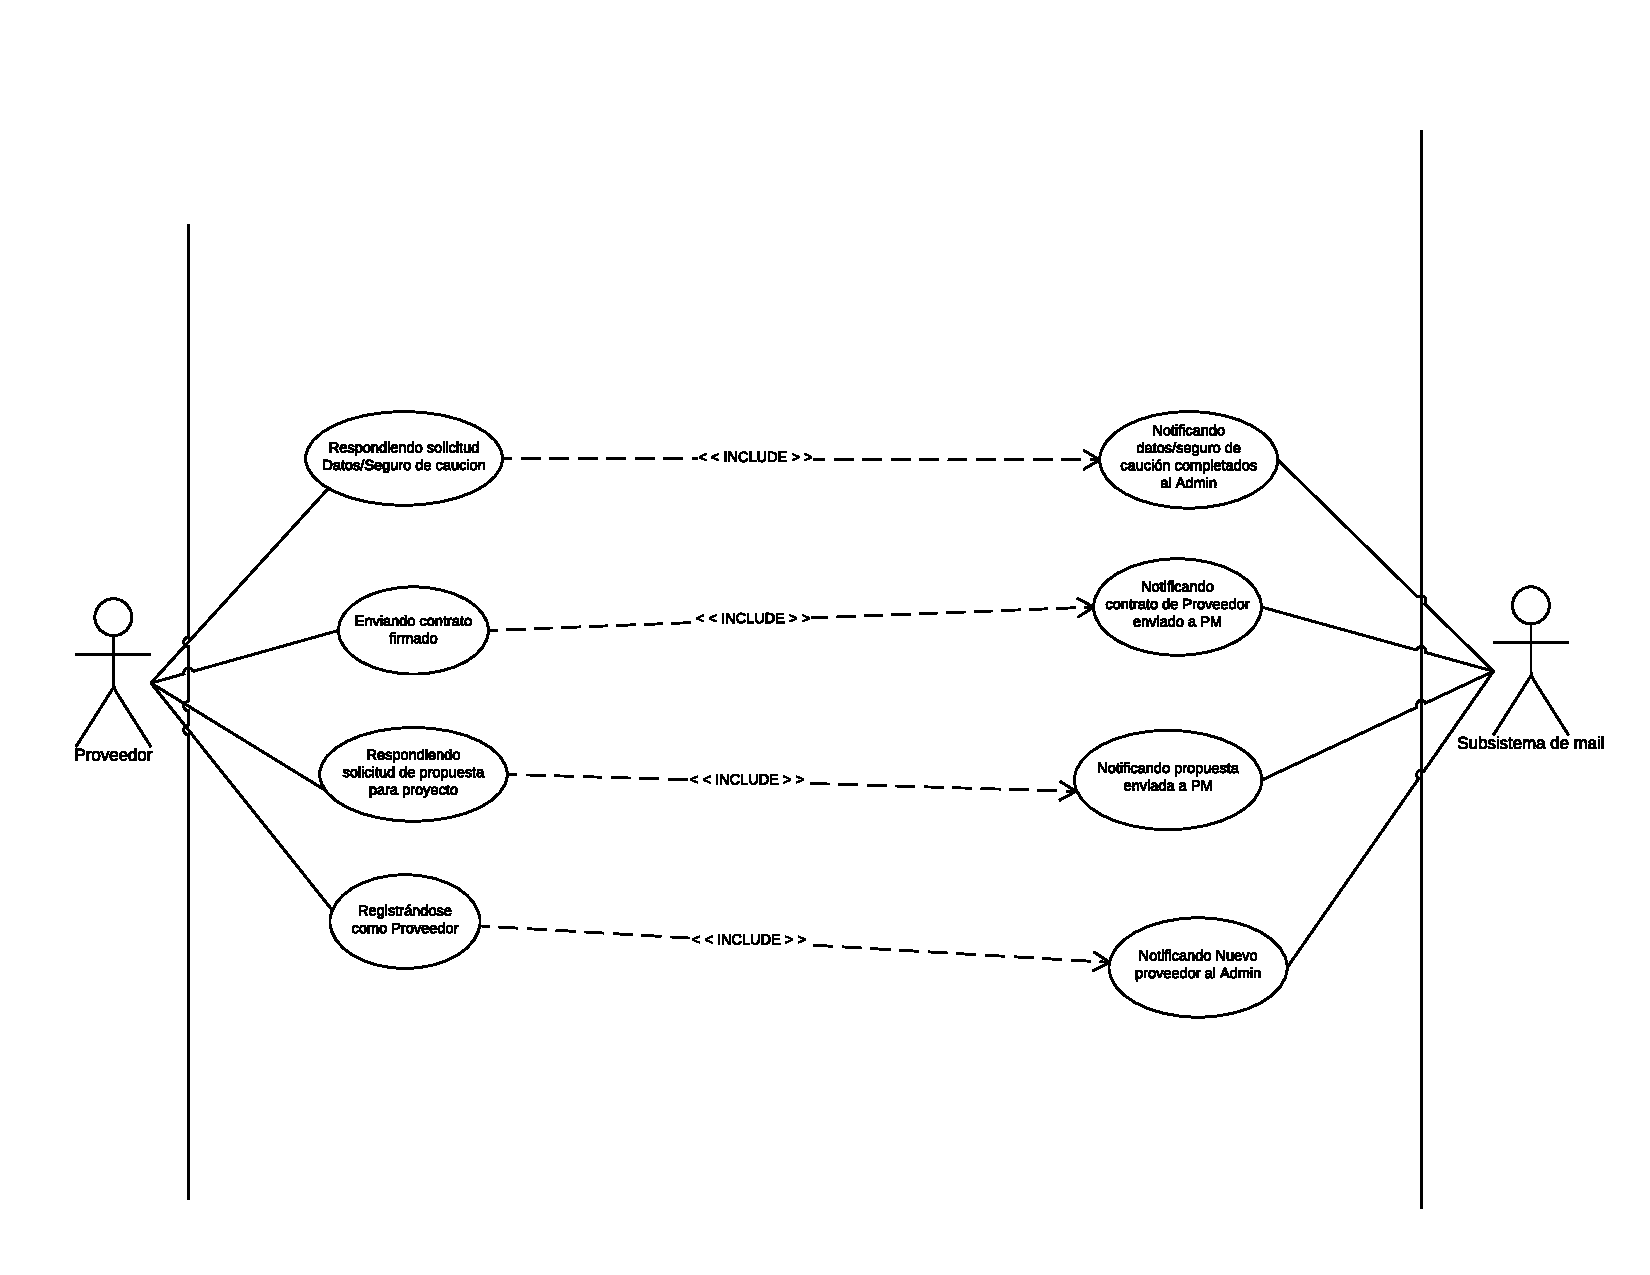
\includegraphics[width=\linewidth]{diag/viejos/cu5.pdf}
\end{figure}
\begin{figure}[H]
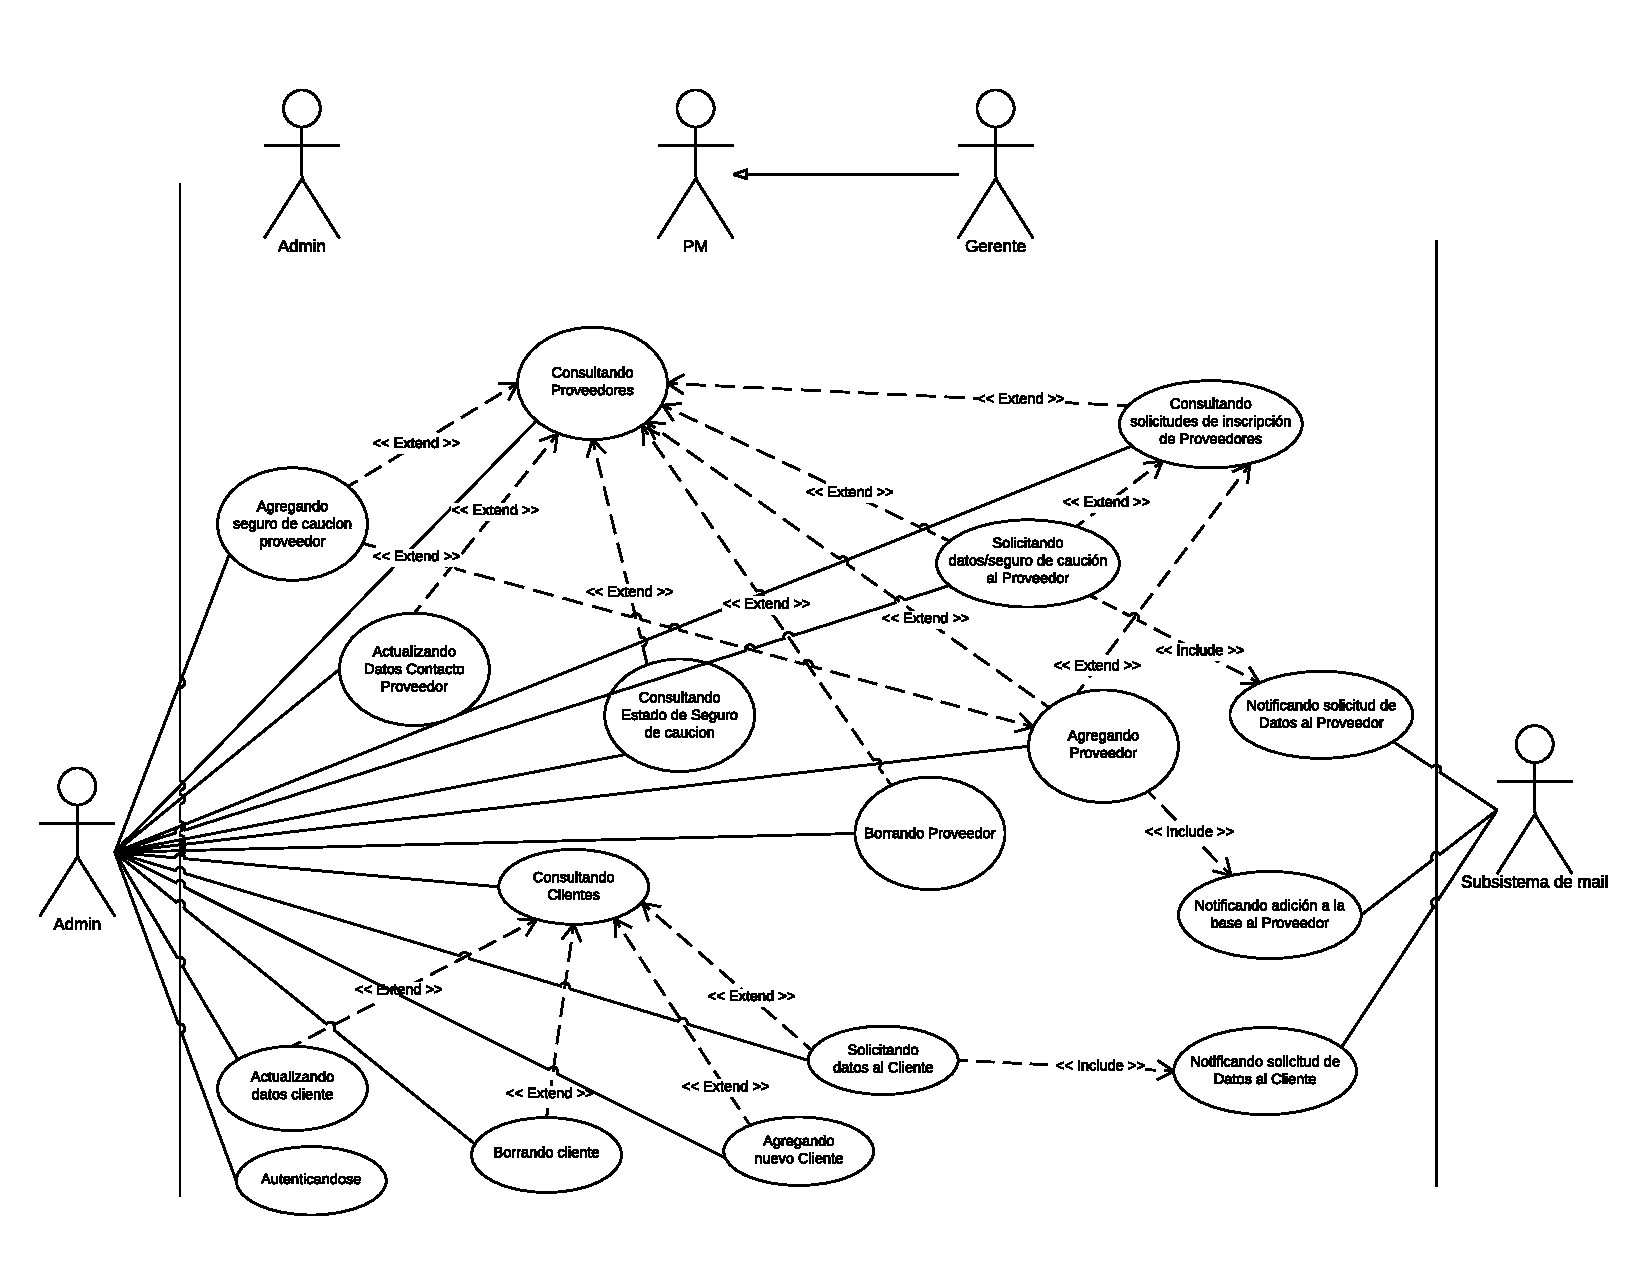
\includegraphics[width=\linewidth]{diag/viejos/cu6.pdf}
\end{figure}

Para finalizar detallaremos los distintos casos de uso en los que ademas intentaremos ver cuales son los comportamientos alternativos que pueda tener nuestro sistema en las distintas sircunstancias.

% ADMIN
\begin{longtable}{| p{.60\textwidth} | p{.40\textwidth} |} 
    \hline
    \multicolumn{2}{|p{16cm}|}{
        \textbf{Caso de uso:} Consultando Proveedores \newline
        \textbf{Actor:} Administrador\newline
        \textbf{Pre:}  True\newline
        \textbf{Post:}El Administrador consulta el proveedor.
    }\\
    \hline
    1.El sistema le solicita que ingrese los filtros de busqueda  & \\
    \hline
    2.El Administrador Agrega los datos del provedor que esta buscando& \\
    \hline
    3.El Sistema encuentra el proveedor y muestra los datos de contacto & 3.1.El proveedor solicitado no se encuentra en el sistema \newline 3.2 Fin de C.U.  \\
    \hline
    4.El Administrador decide elimiar el proveedor. Extiende Caso de uso Borrando Proveedor.& \\
    \hline
    5.El Administrador decide agregar el seguro de Caucion de proveedor. Extiende Caso de uso Agregando Seguro de Caucion.& \\
    \hline
    6.El Administrador decide consultar estado del seguro de Caucion de proveedor. Extiende Caso de uso Consultando estado de seguro de caucion.& \\
    \hline
    7.El Administrador decide actualizar datos del proveedor. Extiende Caso de uso Actualizando datos de proveedor.& \\
    \hline
    8.Fin de C.U.& \\
    \hline
\end{longtable}

\begin{longtable}{| p{.60\textwidth} | p{.40\textwidth} |} 
    \hline
    \multicolumn{2}{|p{16cm}|}{
        \textbf{Caso de uso:} Agregando Proveedor \newline
        \textbf{Actor:} Admin\newline
        \textbf{Pre:}  True\newline
        \textbf{Post:} El proveedor fue agregado al sistema
    }\\
    \hline
    1.El sistema le solicita que ingrese los datos de contacto del proveedor & \\
    \hline
    2.El Administrador Agrega los datos del provedor como son nombres, datos de contacto y datos relacionados al negocio` &  \\
    \hline
    3.El Sistema valida los datos de contacto para ver si no se encuentra registrado & 3.1.El proveedor ya esta dado de alta \newline 3.2 Fin de C.U.  \\
    \hline
    4.El Sistema Pregunta si desea Agregar el seguro de caucion&\\
    \hline
    5.El Administrador Agrega Seguro de caucion, Extiende Caso de Uso Agregar seguro de Caucion. & 5.1 El Administrador decide agregarlo luego. Continua en paso 5 \\
    \hline
    6.El Sistema Guarda el proveedor. USA Notificando adicion a la base de proveedores& \\
    \hline
    7.Fin de C.U.& \\
    \hline
\end{longtable}

\begin{longtable}{| p{.60\textwidth} | p{.40\textwidth} |} 
    \hline
    \multicolumn{2}{|p{16cm}|}{
        \textbf{Caso de uso:} Borrando Proveedor \newline
        \textbf{Actor:} Administrador\newline
        \textbf{Pre:}  Proveedor Seleccionado\newline
        \textbf{Post:} El proveedor fue eliminado del sistema
    }\\
    \hline
    1.El sistema  muetra las opciones para realizar con un proveedor & \\
    \hline
    2.El Administrador selecciona eliminar& \\
    \hline
    3.El Sistema lanza un mensaje consultando si desea eliminar el proveedor &  \\
    \hline
    4.El Administrador selecciona que SI desea eliminar el proveedor & 4.1.1 El Sistema nota que el proveedor sigue asignado a un proyecto en curso, muestra un mensaje por pantalla notificando este problema \newline 4.1.2 Fin Caso de Uso \newline 4.2.1 El usuario Selecciona que NO desea eliminar el proveedor \newline4.2.2 Fin de Caso de uso\\
    \hline
    5.El Sistema elimina el proveedor del sistema &  \\
    \hline
    6.Fin de C.U.& \\
    \hline
\end{longtable}
\begin{longtable}{|p{.60\textwidth}|p{.40\textwidth}|}
    \hline
    \multicolumn{2}{|p{16cm}|}{
        \textbf{Caso de uso:} Actualizando datos de contacto de Proveedor \newline
        \textbf{Actor:} Administrador\newline
        \textbf{Pre:}  Proveedor seleccionado\newline
        \textbf{Post:} El Administrador actualiza los datos del Proveedor
    }\\
    \hline
    1.El sistema  muetra las opciones para realizar con un proveedor & \\
    \hline
    2.El Administrador selecciona Actualizar Datos Proveedor&   \\
    \hline
    3.El Sistema muestra todos los campos con los datos del proveedor para modificar y dos botones , uno para guardar y otro para cancelar&  \\
    \hline
    4.El Administrador Modifica los datos y toca salvar & 4.1.El Administrador toca cancelar \newline 4.2 Fin Caso de Uso \\
    \hline
    5.El Sistema guarda los cambios al proveedor &  \\
    \hline
    6.Fin de C.U.& \\
    \hline
\end{longtable}

\begin{longtable}{|p{.60\textwidth}|p{.40\textwidth}|}
    \hline
    \multicolumn{2}{|p{16cm}|}{
        \textbf{Caso de uso:} Consultando estado de seguro de caucion \newline
        \textbf{Actor:} Administrador\newline
        \textbf{Pre: }  Proveedor seleccionado \newline
        \textbf{Post:} El Administrador consulta estado del seguro de caucion
    }\\
    \hline
    1.El Administrador selecciona la opcion consultar estado de seguro de caucion&  \\
    \hline
    2.El Sistema muestra el estado de seguro de caucion&  \\
    \hline
    3.Fin de C.U.& \\
    \hline
\end{longtable}

\begin{longtable}{|p{.60\textwidth}|p{.40\textwidth}|}
    \hline
    \multicolumn{2}{|p{16cm}|}{
        \textbf{Caso de uso:} Agregando seguro de caucion\newline
        \textbf{Actor:} Administrador\newline
        \textbf{Pre: }  Proveedor seleccionado\newline
        \textbf{Post:} El Administrador Agrega un nuevo seguro de caucion
    }\\
    \hline
    1.El Administrador selecciona la opcion agregar de seguro de caucion& \\
    \hline
    2.El Sistema muestra la opcion de ingreso de validez del seguro de caucion y el ingreso del archivo con el seguro de caucion&  \\
    \hline
    3.El Administrador ingresa la fecha de validez, agrega el archivo del escaneo del seguro de caucion y guarda los cambios&3.1 El administrador Apreta el boton cancelar \newline 3.2 Fin del Caso de uso \\
    \hline
    4.El Sistema verifica la fecha de validez y que no que no exista otro seguro de caucion & \\
    \hline
    5.El Sistema aprueba los datos ingresados y guarda los cambios &5.1.1 Los datos ingresados son incorrectos,el sistema muestra mensaje de error \newline 5.1.2 vuelve al paso 4 \newline 5.2.1 Existe otro seguro de caucion en la misma fecha, el sistema muestra un mensaje avisando que actualizara los datos con el nuevo seguro de caucion. \newline 5.2 vuelve al paso 4\\
    \hline
    6.Fin de C.U.& \\
    \hline
\end{longtable}

\begin{longtable}{|p{.60\textwidth}|p{.40\textwidth}|}
    \hline
    \multicolumn{2}{|p{16cm}|}{
        \textbf{Caso de uso:} Solicitando datos/seguro de caucion de proveedor\newline
        \textbf{Actor:} Administrador\newline
        \textbf{Pre:} Proveedor seleccionado\newline
        \textbf{Post:} El Administrador Agrega un nuevo seguro de caucion
    }\\
    \hline
    1.El sistema  muetra las opciones para realizar con un proveedor & \\
    \hline
    2.El Administrador selecciona la opcion agregar de seguro de caucion& \\
    \hline
    3.El Sistema muestra la opcion de ingreso de validez del seguro de caucion y el ingreso del archivo con el seguro de caucion&  \\
    \hline
    4.El Administrador ingresa la fecha de validez, agrega el archivo del escaneo del seguro de caucion y guarda los cambios&4.1 El administrador Apreta el boton cancelar \newline 4.2 Fin del Caso de uso \\
    \hline
    5.El Sistema verifica la fecha de validez y que no que no exista otro seguro de caucion & \\
    \hline
    6.El Sistema aprueba los datos ingresados y guarda los cambios &6.1 Los datos ingresados son incorrectos, o hay otro seguro de caucion en la misma fecha  \newline 6.2 vuelve al paso 4\\
    \hline
    7.Fin de C.U.& \\
    \hline
\end{longtable}


% cliente

\begin{longtable}{|p{.60\textwidth}|p{.40\textwidth}|}
    \hline
    \multicolumn{2}{|p{16cm}|}{
        \textbf{Caso de uso:} Contactando por nuevos trabajos\newline
        \textbf{Actor:} Cliente\newline
        \textbf{Pre: }  True\newline
        \textbf{Post:} El Cliente deja el contacto para un nuevo trabajo en el sistema
    }\\
    \hline
    1.El Cliente seleccion la opcion de contacto y completa los datos de contacto&2.1 El Cliente no ingresa datos de contacto\newline 1.2 Fin caso de uso   \\
    \hline
    2.El Sistema notifica nuevo proyecto. USA Notificando nuevos trabajos a gerente& \\
    \hline
    3.Fin de C.U.& \\
    \hline
\end{longtable}


\begin{longtable}{|p{.60\textwidth}|p{.40\textwidth}|}
    \hline
    \multicolumn{2}{|p{16cm}|}{
        \textbf{Caso de uso:} Completando Feedback de PM\newline
        \textbf{Actor:} Cliente\newline
        \textbf{Pre: }El Cliente Accede al sistema con link Provisto en alta de proyecto\newline
        \textbf{Post: }El Cliente Completo la encuesta
    }\\
    \hline
    1.El Usuario accede al link que recibio en el Mail y le abre una pagina web con la encuesta a completar & 1.1.El Usuario desestima el mail .\newline 1.2Fin de C.U.\\
    \hline
    2.El Usuario Completa las preguntas sobre rendimiento del PM de la encuesta y agrega recomendaciones en caso de tenerlas&    \\
    \hline
    3.El Usuario Apreta la opcion de enviar el formulario& \\
    \hline
    4.El Sistema Registra la nueva encuesta&\\
    \hline
    5.El Sistema actualiza el puntaje del PM&\\
    \hline
    6.Fin del C.U&\\
    \hline
\end{longtable}

\begin{longtable}{|p{.60\textwidth}|p{.40\textwidth}|}
    \hline
    \multicolumn{2}{|p{16cm}|}{
        \textbf{Caso de uso:} Reportando Problemas\newline
        \textbf{Actor:} Cliente\newline
        \textbf{Pre: }El Cliente Accede al sistema con link Provisto en alta de proyecto\newline
        \textbf{Post: }El Cliente notifico de un problema
    }\\
    \hline
    1.El Usuario entra a la pagina web con el link provisto y selecciona la opcion reportar problema.&\\
    \hline
    2.El Sistema muestra un formulario con espacio para escribir un detalle del problema&    \\
    \hline
    3.El Cliente Completa dicho formulario y selecciona la opcion Enviar& \\
    \hline
    4.El Sistema Registra el problema. Extiende Notificando Problemas en Proyectos a gerentes y PM&\\
    \hline
    5.Fin del C.U&\\
    \hline
\end{longtable}

\begin{longtable}{|p{.60\textwidth}|p{.40\textwidth}|}
    \hline
    \multicolumn{2}{|p{16cm}|}{
        \textbf{Caso de uso:} Enviando Contrato firmado \newline
        \textbf{Actor:} Cliente\newline
        \textbf{Pre: }El Cliente Accede al sistema con link Provisto en alta de proyecto\newline
        \textbf{Post: }El Envio el contrato firmado
    }\\
    \hline
    1.El Usuario entra a la pagina web con el link provisto y selecciona la opcion enviar contrato.&\\
    \hline
    2.El Sistema pide que seleccion el archivo pdf firmado desde su computadora&    \\
    \hline
    3.El Cliente Selecciona el archivo.& \\
    \hline
    4.El Sistema Guarda el contrato firmado. Extiende Notificando contrato de Cliente enviado a PM&\\
    \hline
    5.Fin del C.U&\\
    \hline
\end{longtable}

\begin{longtable}{|p{.60\textwidth}|p{.40\textwidth}|}
    \hline
    \multicolumn{2}{|p{16cm}|}{
        \textbf{Caso de uso:} Respondiendo solicitud de Datos \newline
        \textbf{Actor:} Cliente\newline
        \textbf{Pre: }El Cliente Accede al sistema con link Provisto en mail de solicitud\newline
        \textbf{Post: }El Envio el contrato firmado
    }\\
    \hline
    1.El Usuario entra a la pagina web con el link provisto.&\\
    \hline
    2.El Sistema Presenta un formulario con datos obligatorios como telefono, ubicacion, nombre, datos del negocio, servicios y productos que ofrece &    \\
    \hline
    3.El Cliente Completa los datos y presiona el boton guardar. &3.1 El Cliente no completa los datos.\newline 3.2 El Sistema lo marca como incompleto.\newline 3.3 Fin del C.U.\\
    \hline
    4.El Sistema Guarda los datos. Extiende Notificando datos completados al Admin&\\
    \hline
    5.Fin del C.U&\\
    \hline
\end{longtable}


% PM

\begin{longtable}{|p{.60\textwidth}|p{.40\textwidth}|}
    \hline
    \multicolumn{2}{|p{16cm}|}{
        \textbf{Caso de uso:}Consultando Proyectos\newline
        \textbf{Actor:} PM\newline
        \textbf{Pre: }El PM esta logueado en el sistema\newline
        \textbf{Post:} El PM ve todos los proyectos registrados en el sistema
    }\\
    \hline
    1.El PM selecciona buscar proyectos& \\
    \hline
    2.El sistema muestra todos los proyectos disponibles en forma de lista mostrando nombre del cliente y nombre del proyecto &\\
    \hline
    3.El PM decide filtrar por Cliente y seleccion la opcion de fitlrar por cliente& \\
    \hline
    4.El PM escribe el nombre del Cliente& \\
    \hline
    5.El Sistema lista todos los resultados de busqueda&\\
    \hline
    6.Fin del C.U.&\\
    \hline
\end{longtable}

\begin{longtable}{|p{.60\textwidth}|p{.40\textwidth}|}
    \hline
    \multicolumn{2}{|p{16cm}|}{
        \textbf{Caso de uso:}Consultando alcance de Proyectos\newline
        \textbf{Actor:} PM\newline
        \textbf{Pre: }Proyecto Seleccionado\newline
        \textbf{Post:} El PM Puede ve los alcances de un proyecto
    }\\
    \hline
    1.El Pm Busca un proyecto. Extiende Consultando Proyectos& \\
    \hline
    2.El PM selecciona ver los alcances del proyecto&  \\
    \hline
    3.El sistema muestra los alcances del proyectos& \\
    \hline
    4.Fin del C.U&\\
    \hline
\end{longtable}

\begin{longtable}{|p{.60\textwidth}|p{.40\textwidth}|}
    \hline
    \multicolumn{2}{|p{16cm}|}{
        \textbf{Caso de uso:}Consultando TOP de proveedores\newline
        \textbf{Actor:} PM\newline
        \textbf{Pre: }Proyecto Seleccionado\newline
        \textbf{Post:} El PM obtiene una lista de proveedores ordenados segun los filtros seleccionados
    }\\
    \hline
    1.El sistema muestra los filtros de busqueda como nombre de proveedor, datos del negocio o ubicacion. & \\
    \hline
    2.El PM completa los filtros de busqueda que necesita&  \\
    \hline
    3.El sistema muestra los resultados basado en los filtros de busqueda ordenados por algun criterio seleccionado& \\
    \hline
    4.El PM Selecciona Proveedor &\\
    \hline
    5.El PM Desea enviar una solucitud de presupuesto.Extiende Solictud de propuesta a proveedores &5.1 El PM Desea seguir viendo otros proveedores y presiona el voton retroceder \newline 5.2 Contiuna en el paso 3\\
    \hline
    6.Fin del C.U&\\
    \hline
\end{longtable}


\begin{longtable}{|p{.60\textwidth}|p{.40\textwidth}|}
    \hline
    \multicolumn{2}{|p{16cm}|}{
        \textbf{Caso de uso:}Consultando propuestas de los proveedores\newline
        \textbf{Actor:} PM\newline
        \textbf{Pre: }Proyecto Seleccionado\newline
        \textbf{Post:} El PM obtiene una lista de las propuestas presentadas por los proveedores
    }\\
    \hline
    1.El PM selecciona la opcion de ver propuestas presentadas&\\
    \hline
    2.El sistema muestra las propuestas presentadas por los distintos proveedores & \\
    \hline
    3.El PM selecciona una propuesta  &\\
    \hline
    4.El sistema muestra el detalle de la propuesta seleccionada sobre productos y costos.&4.1 El PM Desea imprimir la propuesta y selecciona boton Imprimir. \newline 4.2. El PM desea volver a la lista de propuestas. Continua en paso 2\\
    \hline
    5.El PM Desea Asignar el proveedor al proyecto. Extiende Asignando proveedor al proyecto.&\\
    \hline
    6.&\\
    \hline
    5.Fin del C.U&\\
    \hline
\end{longtable}

\begin{longtable}{|p{.60\textwidth}|p{.40\textwidth}|}
    \hline
    \multicolumn{2}{|p{16cm}|}{
        \textbf{Caso de uso:}Marcando una propuesta como seleccionada\newline
        \textbf{Actor:} PM\newline
        \textbf{Pre: }Proyecto Seleccionado\newline
        \textbf{Post:} El PM selecciona una de las propeustas para el proyecto seleccionado
    }\\
    \hline
    1.El PM selecciona una propuesta para el proyecto y guarda los cambios&\\
    \hline
    2.El sistema envia una notificacion al proeedor.USA Notificando seleccion de propuesta a proveedor& 2.1 El Proveedor no notifica como recibida la notificacion \newline 2.2 el Sistema no marca como seleccionada la propuesta\\
    \hline
    3.Fin del C.U&\\
    \hline
\end{longtable}

\begin{longtable}{|p{.60\textwidth}|p{.40\textwidth}|}
    \hline
    \multicolumn{2}{|p{16cm}|}{
        \textbf{Caso de uso:}Generando reporte de proyecto\newline
        \textbf{Actor:} PM\newline
        \textbf{Pre: }Proyecto Seleccionado\newline
        \textbf{Post:} El PM agrega un detalle de los avances en el proyecto
    }\\
    \hline
    1.El PM selecciona la opcion de agregar reporte &\\
    \hline
    2.El sistema muestra las un formulario para completar con detalles de tareas y fecha, ademas puede asignar un de estado como critico, con complicaciones o estable& \\
    \hline
    3.El PM completa un formulario con los avances del proyecto y guarda el reporte&\\
    \hline
    4.El sistema guarda el formulario&\\
    \hline
    5.Fin del C.U&\\
    \hline
\end{longtable}


\begin{longtable}{|p{.60\textwidth}|p{.40\textwidth}|}
    \hline
    \multicolumn{2}{|p{16cm}|}{
        \textbf{Caso de uso:}Enviando solicitud de propuesta a proveedores\newline
        \textbf{Actor:} PM\newline
        \textbf{Pre: }Proyecto Seleccionado\newline
        \textbf{Post:} El PM envia la soliicitud de propuestas a los mejores proveedores
    }\\
    \hline
    1.El sistema muestra la lista de TOP de proveedores & \\
    \hline
    2.El PM selecciona varios proveedores y selecciona la opcion de enviar solicitud de propuesta& \\
    \hline
    3.El sistema envia la notificacion.USA Notificando solicitud de porpuestas a proveedores& \\
    \hline
    4.Fin del C.U&\\
    \hline
\end{longtable}

% GERENTE
\begin{longtable}{|p{.60\textwidth}|p{.40\textwidth}|}
    \hline
    \multicolumn{2}{|p{16cm}|}{
        \textbf{Caso de uso:}Asignando PM Al Proyecto\newline
        \textbf{Actor:} Gerente\newline
        \textbf{Pre: }true\newline
        \textbf{Post:} Un PM es asignado al proyecto
    }\\
    \hline
    1.El Gerente ingresa al sistema & \\
    \hline
    2.El Gerente Consulta los proyectos nuevos en el sistema USA Consultando Nuevos Trabajos&    \\
    \hline
    3.El Gerente Consulta los mejores PM para el proyecto dado USA Consutlando TOP Proveedores& \\
    \hline
    4.El Gerente Asigna el mejor PM Al Proyecto&\\
    \hline
    5.Fin del C.U&\\
    \hline
\end{longtable}


\begin{longtable}{|p{.60\textwidth}|p{.40\textwidth}|}
    \hline
    \multicolumn{2}{|p{16cm}|}{
        \textbf{Caso de uso:}Consultando Reportes de proyecto\newline
        \textbf{Actor:} Gerente\newline
        \textbf{Pre: }true\newline
        \textbf{Post:}  El Gerente Consulta el estado de un proyecto
    }\\
    \hline
    1.El Gerente ingresa al sistema & \\
    \hline
    2.El Gerente Busca un proyecto segun ciertos filtros. Extiende Consultando Proyectos&    \\
    \hline
    3.El Sistema le devuelve una lista de proyectos& \\
    \hline
    4.El Gerente Selecciona un proyecto y presiona el boton de obtener estado de proyecto&\\
    \hline
    5.El Sistema Devuelve el estado del proyecto seleccionado &\\
    \hline
    6.Fin del C.U.&\\
    \hline
\end{longtable}



\appendix
%\include{apendice}

\bibliographystyle{plain}
%\bibliography{tp2}

\end{document}
